\section{What survives}
\label{sec:survives}

The MoE-matched comparison shows DG's advantage is concentrated at
serial mode. DG wins at every practical output length. The five
conditions that define the regime where block diffusion is the right
choice are:
\begin{enumerate}[nosep]
  \item Output length $\geq 7$ tokens (DG crossover in serial mode).
  \item Batch-1 by requirement: tenant isolation, interactivity, or
    serial chain structure.
  \item Completeness is validated against a schema.
  \item The quality floor exceeds what the AR model delivers.
  \item A \dgWeights\,GB resident footprint is acceptable.
\end{enumerate}

\paragraph{Why serial investigation chains are the natural habitat of the staircase.}

A security operations centre receives an alert, looks up threat
intelligence, cross-references internal logs, and drills into the next
layer. Each hop blocks on the previous; concurrency is 1 by
construction. Against AR-30B, DG is roughly fourteen times faster per
hop --- the chain harness measures DG at 419\,ms per hop rather than
the 379\,ms anchor, because each hop re-prefills a longer accumulated
prompt. The gap widens in absolute terms with depth: at eight hops, the
difference between three seconds and forty-seven seconds is the
difference between catching an intruder in the act and finding the
trail gone cold. Figure~\ref{fig:chains} shows that neither the
per-hop cost nor DG's tail penalty grows with depth.

\begin{figure}[!htbp]
\centering
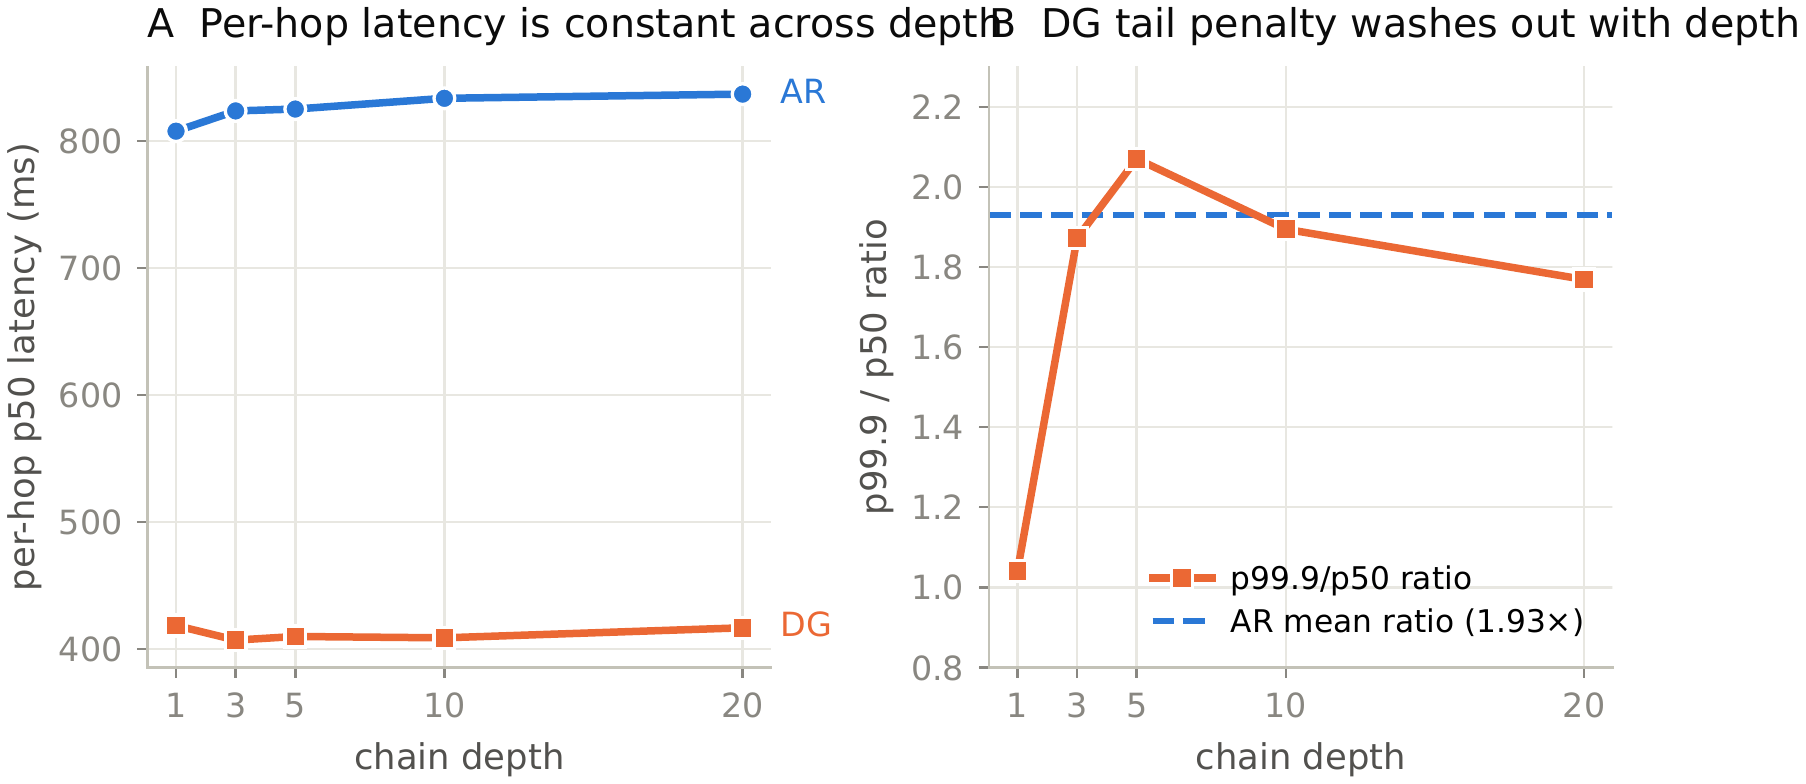
\includegraphics[width=\linewidth]{figures/fig10_usecase_chains_hires.png}
\caption{Serial investigation chains. \textbf{A:} per-hop p50 is
constant across depth --- the staircase does not steepen. \textbf{B:}
the AR/DG latency ratio at p99.9 climbs from $1.04\times$ at one hop
to the median ratio ($\sim$$1.9\times$) by ten hops. DG's fat tail
almost erases its advantage on a single hop, but independent hops
average out, so the longer the chain the more of its median advantage
DG keeps (BGL, $n{=}300$, $K{=}8$; AR arm is the dense AR-3B
baseline).}
\label{fig:chains}
\end{figure}

\paragraph{What happens when a deadline expires mid-generation?}

A FATAL log line arrives mid-stream. DG's bounded service time and
complete-canvas guarantee make it suitable for priority preemption: a
preempted request returns a valid record, not a truncated one. The AR
model, interrupted mid-generation, returns half a JSON object ---
syntactically invalid, unusable downstream. In a system that must
decide whether to page an on-call engineer at 3\,a.m., the difference
between a complete record and a truncated one is the difference
between an actionable alert and a false negative.

The $K$ knob is DG's emergency brake: when a deadline tightens, drop
$K$ from 8 to 4 and the model still fills every field --- just with
slightly less precision --- instead of cutting the JSON in half
mid-key. AR has no equivalent; its only response to a deadline is
truncation. The completeness guarantee holds only above the canvas
length; below $L{=}128$ DG's schema validity collapses to
\dgValidTwentyEight\% against AR's \arValidTwentyEight\%
(Appendix~\ref{app:quality}). Graceful degradation is a property of
the \emph{time} budget, not the output-length budget.

\paragraph{Why autonomous driving is batch-1 by construction.}

One vehicle, one scene, one decision. There is no batching a braking
decision --- the car either processes the scene or it does not. The
$K$ knob is a per-request quality slider: drop $K$ to meet a tightened
deadline without truncating output. Output is long --- multi-object
scene description, predicted trajectories --- which is exactly where
the staircase advantage is largest.

\paragraph{Why algorithmic trading rewards long chains.}

A serial chain with a 1--5\,s market reaction window. At eight or more
hops, DG's staircase advantage provides faster end-to-end analysis.
The taxi fare compounds; the subway fare does not.

\paragraph{Why wide schemas favour joint denoising.}

DG's joint-canvas denoising treats all fields as one structured
object. Across schema widths from 12 to 100 fields, DG's latency
advantage held at roughly two- to threefold
(Figure~\ref{fig:schema}; measured against the dense AR-3B baseline,
not AR-30B).

\begin{figure}[!htbp]
\centering
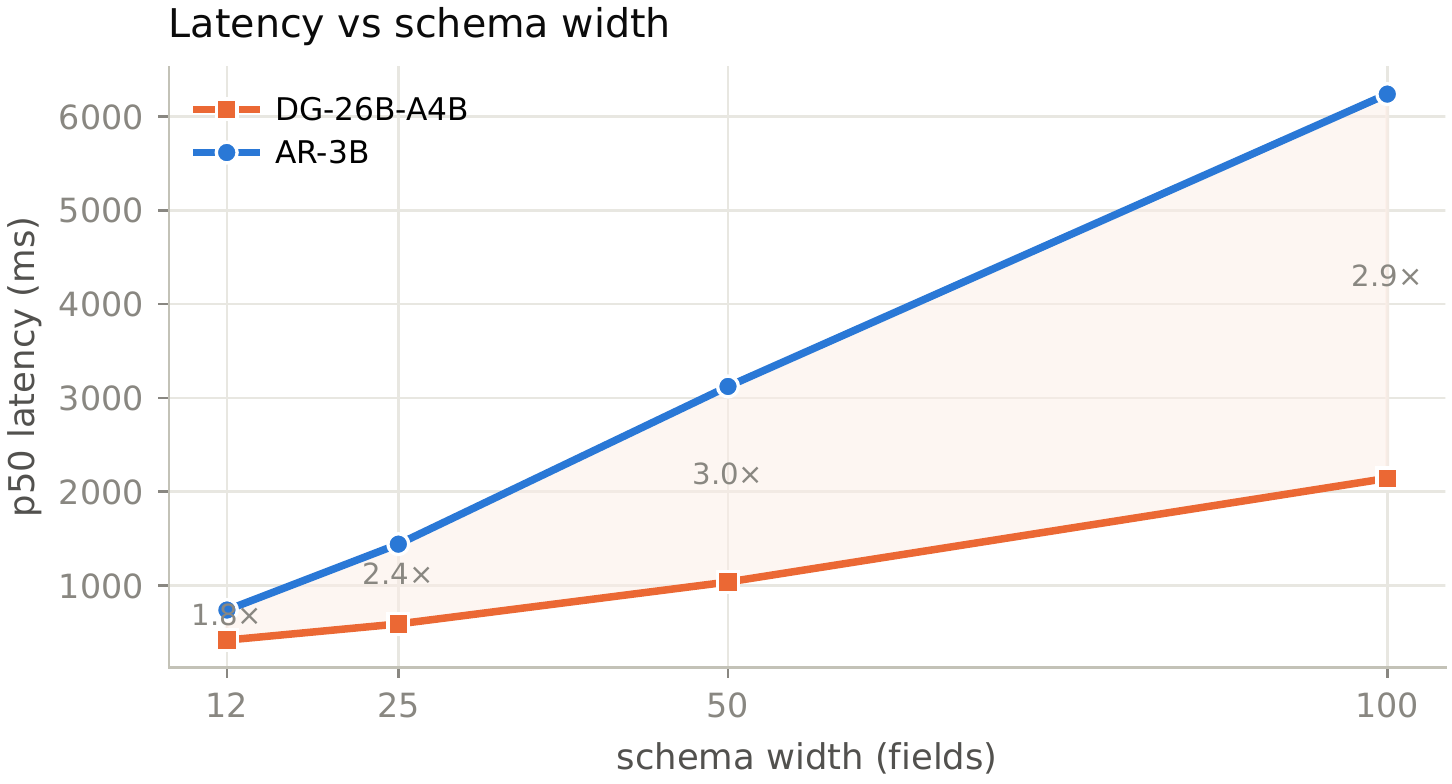
\includegraphics[width=0.85\linewidth]{figures/fig11_usecase_schema_hires.png}
\caption{Latency vs schema width (BGL, $n{=}300$). DG's advantage
holds across widths because all fields are denoised in one canvas.}
\label{fig:schema}
\end{figure}

\paragraph{Where diffusion does not win.}

High-rate log streams favour AR's batching advantage. Tail-sensitive
single-stream workloads with strict p99 SLAs are hurt by DG's
max/median ratio. And any workload that can batch favours AR
regardless of output length.

\paragraph{Where diffusion fails.}

Six hypotheses about diffusion's structural advantages were tested and
refuted; see Appendix~\ref{app:refuted}. The most instructive failures:
bidirectional attention propagates input noise in both directions,
making DG \emph{less} robust to perturbation than AR in all ten tested
categories. DG's joint denoising should preserve suffix tokens by
construction, but AR trivially regenerates the whole record from the
prompt. And selective re-masking gains a small F1 improvement over
three rounds, but still trails AR after a single pass. These failures
define the operational boundary: block diffusion's advantage is in
\emph{latency shape at long output}, not in robustness, infilling, or
iterative refinement.

\FloatBarrier
